\documentclass{article}
%Preamble
\usepackage{float}
\usepackage{color}
\usepackage{listings}
\usepackage{longtable}
\usepackage{amsmath,amssymb}
\usepackage{graphics}
\usepackage{graphicx}

\title{AE 622 -  Computing of high speed flows\\ Assignment 4: Report \\ Shock waves generated by 2D wedge}
\author{Vinod Kumar Metla - 130010048\\Aditi Taneja - 13D100026}
\date{\today}

\begin{document}
\pagenumbering{arabic}
\maketitle
\newpage
\section*{Introduction}
Oblique shock waves are generated by sharp two-dimensional wedges. Free Stream mach number is taken as 2.0 and weak shock turn angle as $20^o$. Two grid sizes - 200x50 and 200x100 are used to compute the solution and compared with the wave angle obtained from $\theta-\beta-M $ relation.
CFL number is varied to obtain the optimal cfl value for which residue is minimum.
Following CFL values were tried and residue vs. number of iterations plots were compared.
\begin{enumerate}
\item 0.01
\item 0.05
\item 0.1
\item 0.2
\item 0.4
\item 0.5

\end{enumerate}

Simulations are carried out for 30,000 iterations on both grid sizes.

\section*{Dependencies}
\begin{enumerate}
\item Pdflatex 
\item Numpy
\item Matplotlib

\end{enumerate}
\newpage

\section*{Plots with ymax= 1.0 , xmax = 0.5}
\subsection*{200x50 Grid}
\begin{figure}[H]   \label{figure}
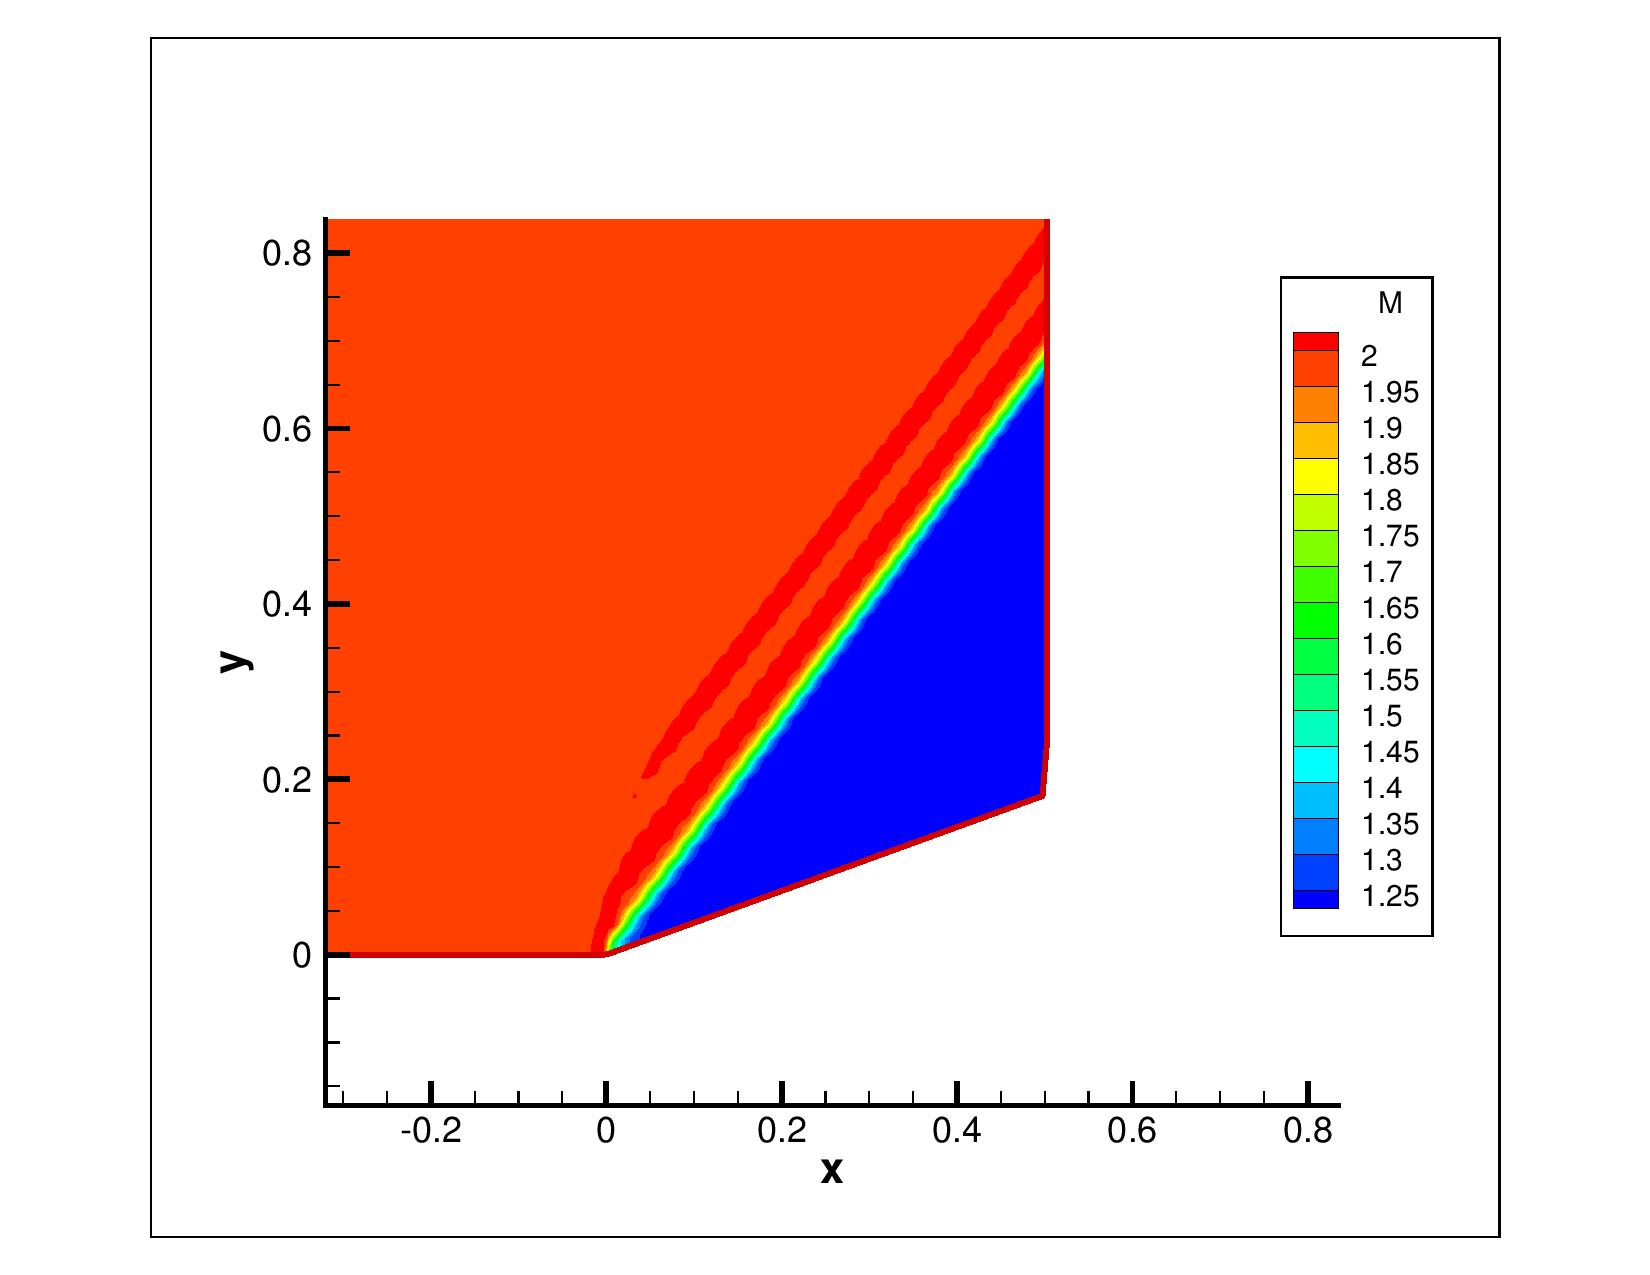
\includegraphics[width=14cm]{200x50/grid50.jpg}		%%%%%%%%%%%change location and name
\label{figure:}
\caption{Contour Plot for Mach Number on 200x50 grid after 30,000 iterations}
\end{figure}
\newpage

\subsection*{200x100 Grid with ymax= 1.0 , xmax = 0.5}
\begin{figure}[H]   \label{figure}
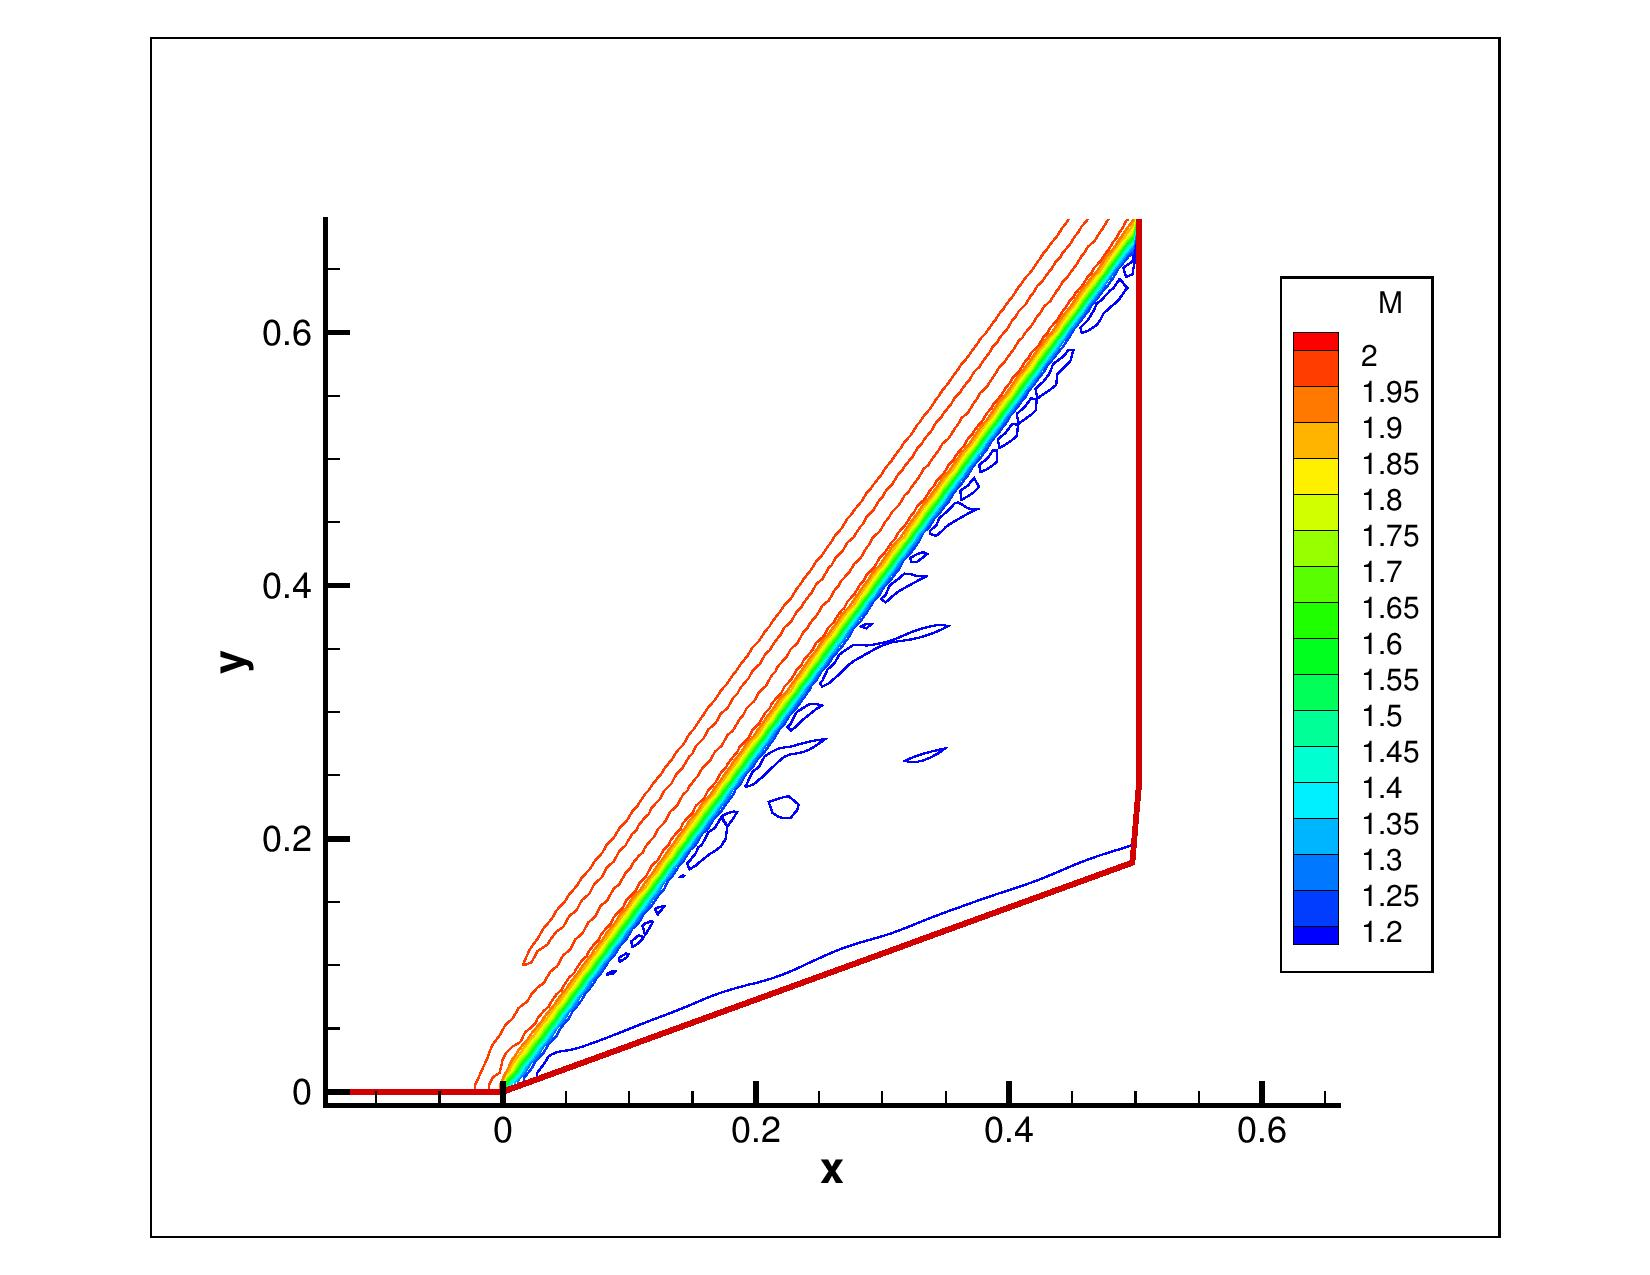
\includegraphics[width=15cm]{200x100/grid100.jpg}		%%%%%%%%%%%change location and name
\label{figure:}
\caption{Contour Plot for Mach Number on 200x100 grid after 30,000 iterations}
\end{figure}

\subsection*{200x50 Grid with ymax= 1.0 , xmax = 0.5 }
\begin{figure}[H]   \label{figure}
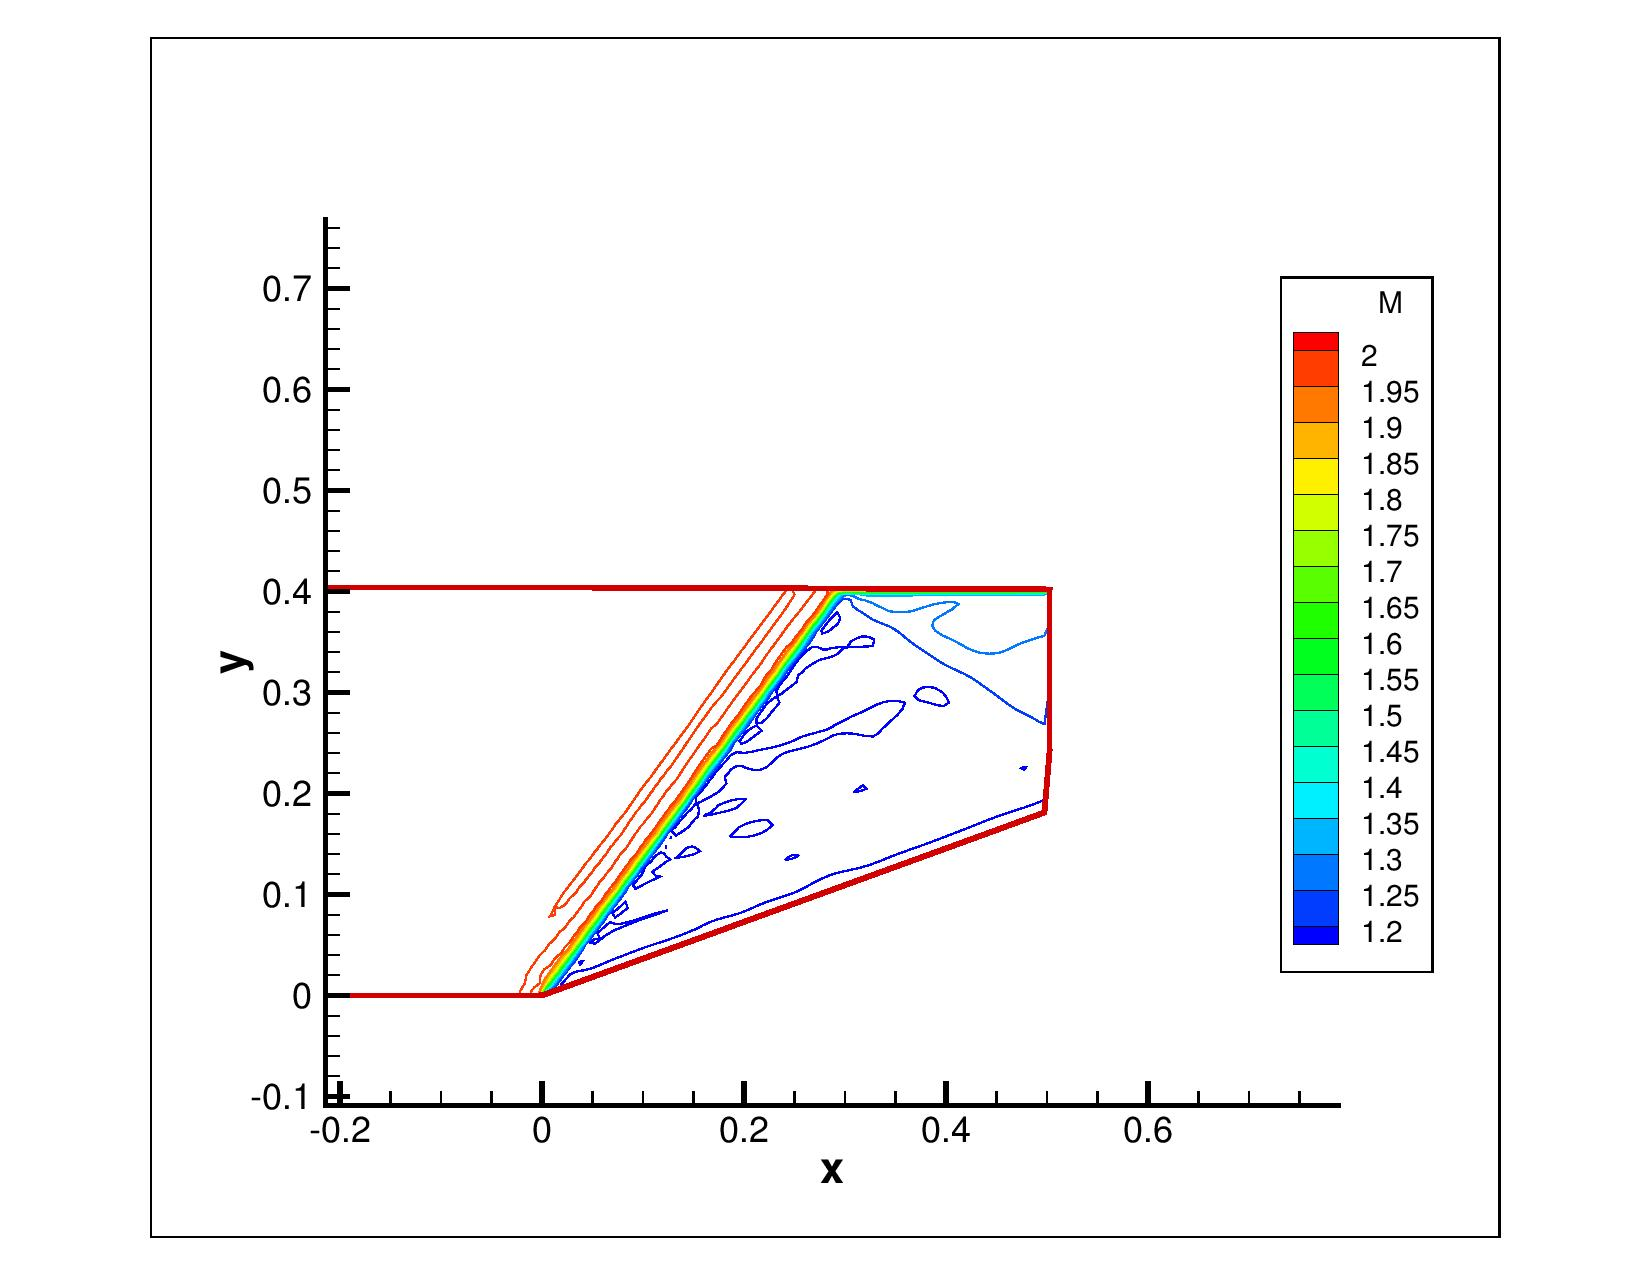
\includegraphics[width=14cm]{05x04/grid50.jpg}		%%%%%%%%%%%change location and name
\label{figure:}
\caption{Contour Plot for Mach Number on 200x50 grid after 30,000 iterations}
\end{figure}
\newpage


\newpage
\subsection*{Residue Plot comparing different grid sizes}
\begin{figure}[H]   \label{figure}
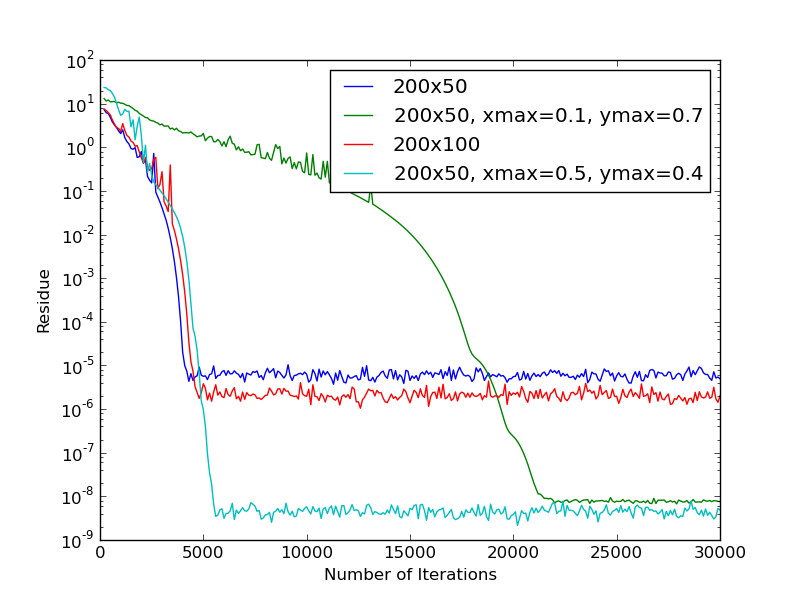
\includegraphics[width=15cm]{residue.png}		%%%%%%%%%%%change location and name
\label{figure:}
\caption{Plot for Comparison of Residue vs. Number of Iterations for two grid sizes.}
\end{figure}

\newpage
\subsection*{Residue Plots for different CFL number on 200x50 grid}
\begin{figure}[H]   \label{figure}
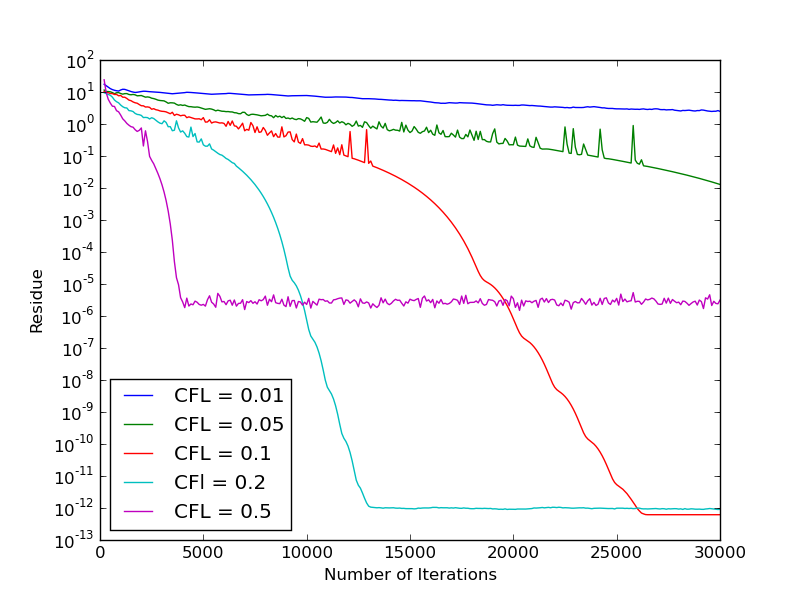
\includegraphics[width=15cm]{residue1.png}		%%%%%%%%%%%change location and name
\label{figure:}
\caption{Plot for Comparison of Residue vs. Number of Iterations for different CFL number}
\end{figure}


\newpage
\subsection*{Density Plot for calculating Shock width}
Oblique shock width was calculated by plotting density vs. x for a streamline passing through the shock with free stream Mach Number = 2.0, x domain = 0.5, y domain = 1.0, 200x50 grid Size.
\begin{figure}[H]   \label{figure}
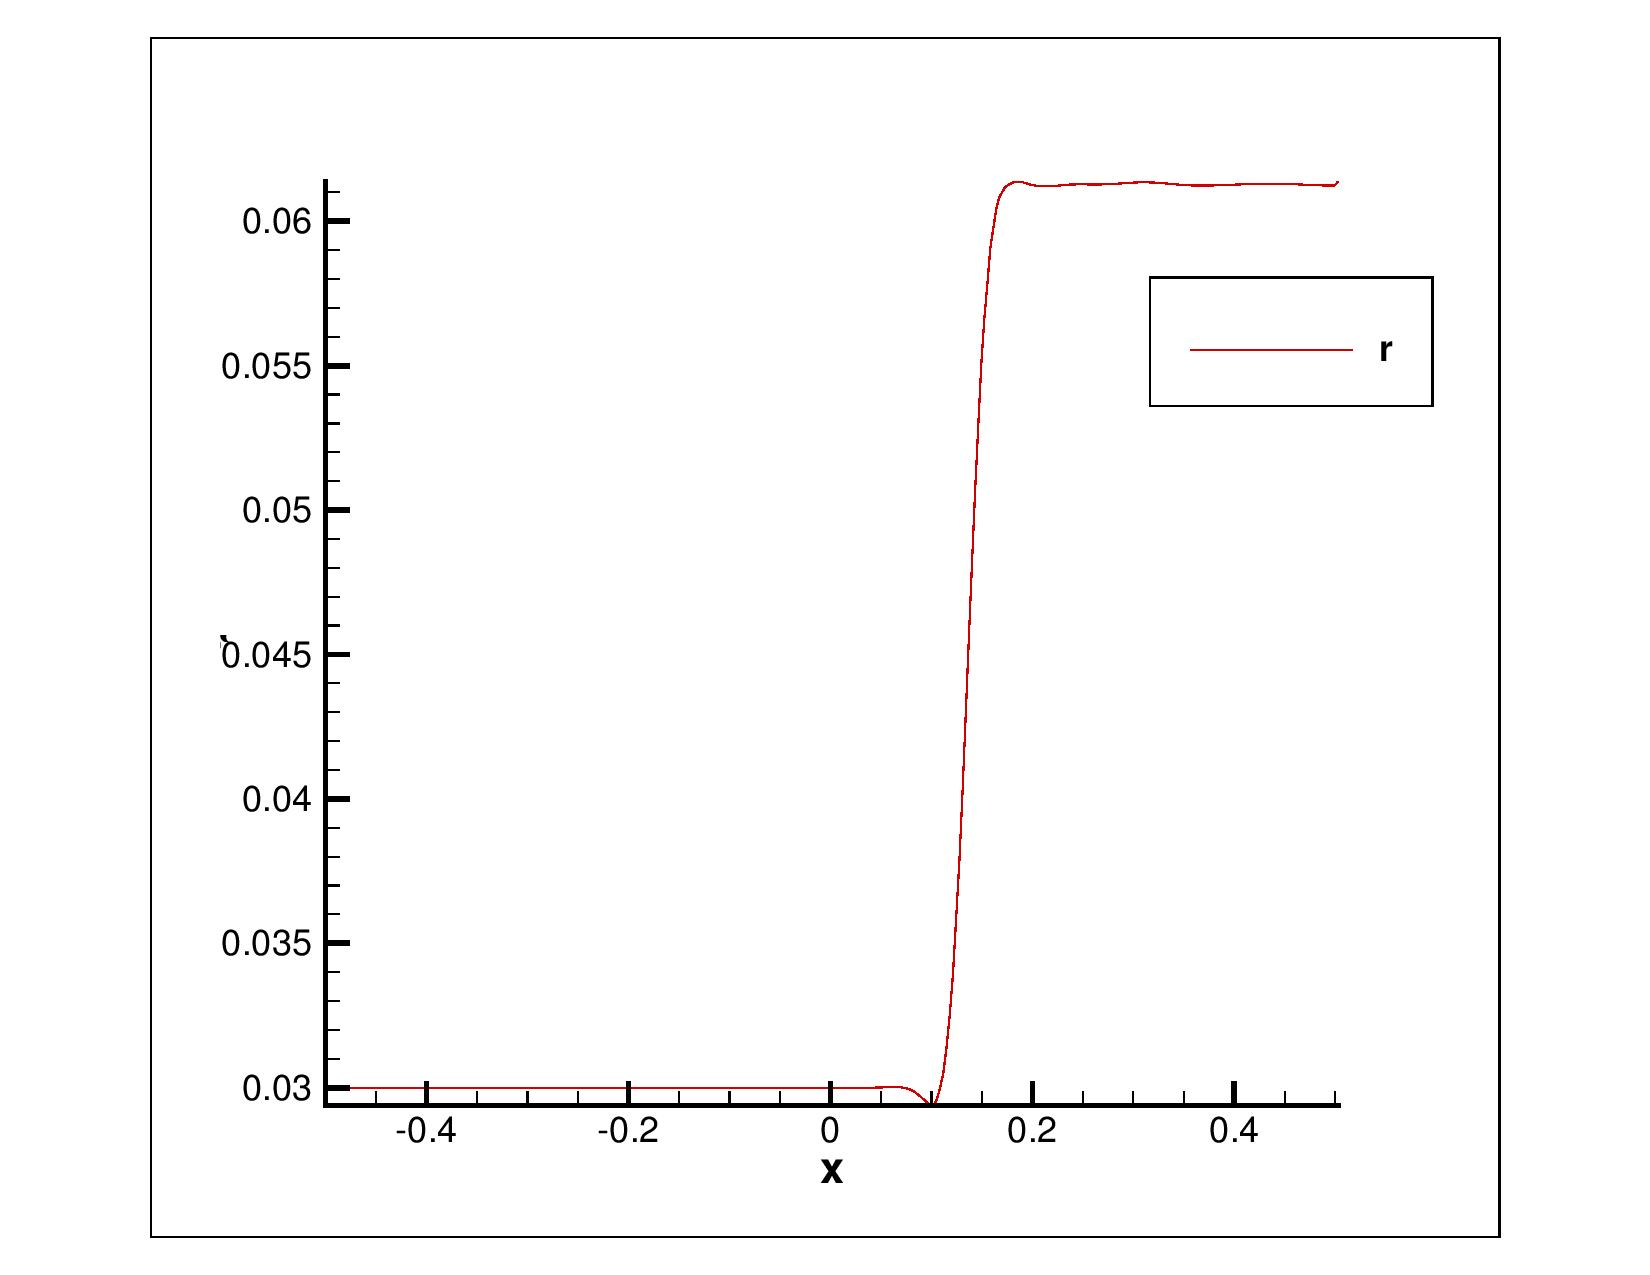
\includegraphics[width=15cm]{200x50/density.jpg}		%%%%%%%%%%%change location and name
\label{figure:}
\caption{Density vs. x for a streamline passing through the oblique shock.}
\end{figure}

\newpage
\section*{Observations}
Different domain sizes and grid sizes were tried and the following observations were made -
\begin{enumerate}
\item For 200x50 grid Size, shock width was obtained to be approx. $8.35 cms$. For 200x100 grid size, shock width obtained is approximately 3.93 cms. Thus, shock width decreased by more than half when grid size was doubled in one direction.
\item Exact Angle obtained from $\theta-\beta-M calculator$ (inviscid theory) for $20^o$ and M =2.0 is $53.4229405^o$ which is close to the approximate angle obtained with 200x50 grid size viz. $52.0121^o$ and with 200x100 grid size = $52.9134^o$. Thus there is a slight improvement in angle from 200x50 grid to 200x100 grid.
\item Residue after 30,000 decreases as ymax is decreased as evident from Figure 4. However, once ymax is decreased beyond a limit, the solution never converges as can be seen from Figure 3. The shock bends along with the top of the grid.
\item It can be concluded that due to numerical errors, significant shock width is observed for all the cases. Stair Effect is visible in the shock because the shock doesn't fit completely in the grid.
\item Variation of Mach number is also observed ahead of the shock instead of a single value (For eg. in Figure 2). This happens mainly due to the presence of numerical errors involved in computations.
\item Not much difference is observed in convergence of the scheme for two grid sizes - 200x50 and 200x100 as can be seen from figure 4. Thus, it is optimal to choose 200x50 grid since the number of computations involved will be less.
\item From figure 5, it can be concluded that as CFL number increases, residue decreases upto certain value and then starts increasing. Also, as CFl number increases convergence rate increases.
\item In figure 4, as the grid domain size is decreased to 0.5x0.4, residue decreases but the solution obtained is wrong.
\item BEST SOLUTION (Minimum residue and least shock width) can be obtained for grid size - 200x100 with ymax= 1.0, x = 0.5, anf CFL number varying from 0.5 (high convergence rate - till 3000 iterations) to 0.2 (after 3000 iterations - less residue).
\end{enumerate}

\subsection*{Residue Plot for optimal CFL number on 200x50 grid}
\begin{figure}[H]   \label{figure}
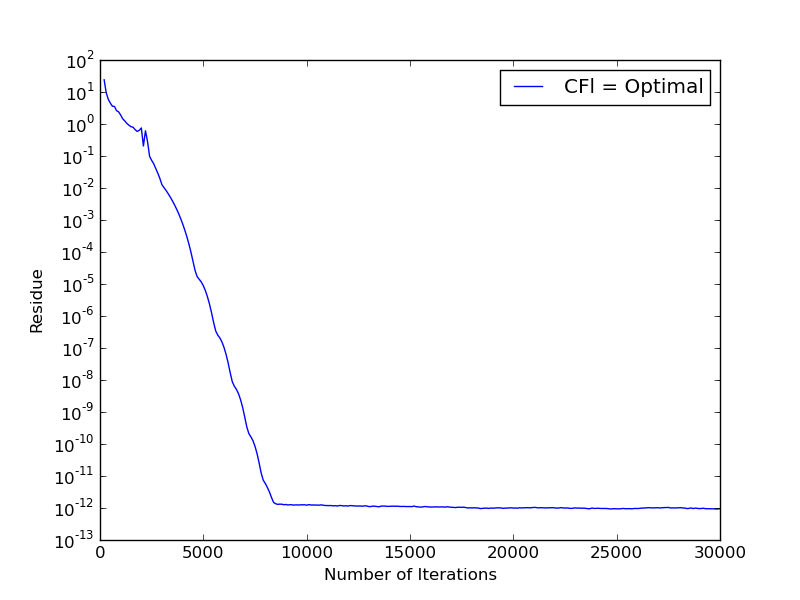
\includegraphics[width=15cm]{best.png}		%%%%%%%%%%%change location and name
\label{figure:}
\caption{Plot of Residue vs. Number of Iterations for optimal CFL number}
\end{figure}


\end{document}
